% Options for packages loaded elsewhere
\PassOptionsToPackage{unicode}{hyperref}
\PassOptionsToPackage{hyphens}{url}
\PassOptionsToPackage{dvipsnames,svgnames,x11names}{xcolor}
%
\documentclass[
  letterpaper,
  DIV=11,
  numbers=noendperiod]{scrartcl}

\usepackage{amsmath,amssymb}
\usepackage{iftex}
\ifPDFTeX
  \usepackage[T1]{fontenc}
  \usepackage[utf8]{inputenc}
  \usepackage{textcomp} % provide euro and other symbols
\else % if luatex or xetex
  \usepackage{unicode-math}
  \defaultfontfeatures{Scale=MatchLowercase}
  \defaultfontfeatures[\rmfamily]{Ligatures=TeX,Scale=1}
\fi
\usepackage{lmodern}
\ifPDFTeX\else  
    % xetex/luatex font selection
\fi
% Use upquote if available, for straight quotes in verbatim environments
\IfFileExists{upquote.sty}{\usepackage{upquote}}{}
\IfFileExists{microtype.sty}{% use microtype if available
  \usepackage[]{microtype}
  \UseMicrotypeSet[protrusion]{basicmath} % disable protrusion for tt fonts
}{}
\makeatletter
\@ifundefined{KOMAClassName}{% if non-KOMA class
  \IfFileExists{parskip.sty}{%
    \usepackage{parskip}
  }{% else
    \setlength{\parindent}{0pt}
    \setlength{\parskip}{6pt plus 2pt minus 1pt}}
}{% if KOMA class
  \KOMAoptions{parskip=half}}
\makeatother
\usepackage{xcolor}
\setlength{\emergencystretch}{3em} % prevent overfull lines
\setcounter{secnumdepth}{5}
% Make \paragraph and \subparagraph free-standing
\makeatletter
\ifx\paragraph\undefined\else
  \let\oldparagraph\paragraph
  \renewcommand{\paragraph}{
    \@ifstar
      \xxxParagraphStar
      \xxxParagraphNoStar
  }
  \newcommand{\xxxParagraphStar}[1]{\oldparagraph*{#1}\mbox{}}
  \newcommand{\xxxParagraphNoStar}[1]{\oldparagraph{#1}\mbox{}}
\fi
\ifx\subparagraph\undefined\else
  \let\oldsubparagraph\subparagraph
  \renewcommand{\subparagraph}{
    \@ifstar
      \xxxSubParagraphStar
      \xxxSubParagraphNoStar
  }
  \newcommand{\xxxSubParagraphStar}[1]{\oldsubparagraph*{#1}\mbox{}}
  \newcommand{\xxxSubParagraphNoStar}[1]{\oldsubparagraph{#1}\mbox{}}
\fi
\makeatother

\usepackage{color}
\usepackage{fancyvrb}
\newcommand{\VerbBar}{|}
\newcommand{\VERB}{\Verb[commandchars=\\\{\}]}
\DefineVerbatimEnvironment{Highlighting}{Verbatim}{commandchars=\\\{\}}
% Add ',fontsize=\small' for more characters per line
\usepackage{framed}
\definecolor{shadecolor}{RGB}{241,243,245}
\newenvironment{Shaded}{\begin{snugshade}}{\end{snugshade}}
\newcommand{\AlertTok}[1]{\textcolor[rgb]{0.68,0.00,0.00}{#1}}
\newcommand{\AnnotationTok}[1]{\textcolor[rgb]{0.37,0.37,0.37}{#1}}
\newcommand{\AttributeTok}[1]{\textcolor[rgb]{0.40,0.45,0.13}{#1}}
\newcommand{\BaseNTok}[1]{\textcolor[rgb]{0.68,0.00,0.00}{#1}}
\newcommand{\BuiltInTok}[1]{\textcolor[rgb]{0.00,0.23,0.31}{#1}}
\newcommand{\CharTok}[1]{\textcolor[rgb]{0.13,0.47,0.30}{#1}}
\newcommand{\CommentTok}[1]{\textcolor[rgb]{0.37,0.37,0.37}{#1}}
\newcommand{\CommentVarTok}[1]{\textcolor[rgb]{0.37,0.37,0.37}{\textit{#1}}}
\newcommand{\ConstantTok}[1]{\textcolor[rgb]{0.56,0.35,0.01}{#1}}
\newcommand{\ControlFlowTok}[1]{\textcolor[rgb]{0.00,0.23,0.31}{\textbf{#1}}}
\newcommand{\DataTypeTok}[1]{\textcolor[rgb]{0.68,0.00,0.00}{#1}}
\newcommand{\DecValTok}[1]{\textcolor[rgb]{0.68,0.00,0.00}{#1}}
\newcommand{\DocumentationTok}[1]{\textcolor[rgb]{0.37,0.37,0.37}{\textit{#1}}}
\newcommand{\ErrorTok}[1]{\textcolor[rgb]{0.68,0.00,0.00}{#1}}
\newcommand{\ExtensionTok}[1]{\textcolor[rgb]{0.00,0.23,0.31}{#1}}
\newcommand{\FloatTok}[1]{\textcolor[rgb]{0.68,0.00,0.00}{#1}}
\newcommand{\FunctionTok}[1]{\textcolor[rgb]{0.28,0.35,0.67}{#1}}
\newcommand{\ImportTok}[1]{\textcolor[rgb]{0.00,0.46,0.62}{#1}}
\newcommand{\InformationTok}[1]{\textcolor[rgb]{0.37,0.37,0.37}{#1}}
\newcommand{\KeywordTok}[1]{\textcolor[rgb]{0.00,0.23,0.31}{\textbf{#1}}}
\newcommand{\NormalTok}[1]{\textcolor[rgb]{0.00,0.23,0.31}{#1}}
\newcommand{\OperatorTok}[1]{\textcolor[rgb]{0.37,0.37,0.37}{#1}}
\newcommand{\OtherTok}[1]{\textcolor[rgb]{0.00,0.23,0.31}{#1}}
\newcommand{\PreprocessorTok}[1]{\textcolor[rgb]{0.68,0.00,0.00}{#1}}
\newcommand{\RegionMarkerTok}[1]{\textcolor[rgb]{0.00,0.23,0.31}{#1}}
\newcommand{\SpecialCharTok}[1]{\textcolor[rgb]{0.37,0.37,0.37}{#1}}
\newcommand{\SpecialStringTok}[1]{\textcolor[rgb]{0.13,0.47,0.30}{#1}}
\newcommand{\StringTok}[1]{\textcolor[rgb]{0.13,0.47,0.30}{#1}}
\newcommand{\VariableTok}[1]{\textcolor[rgb]{0.07,0.07,0.07}{#1}}
\newcommand{\VerbatimStringTok}[1]{\textcolor[rgb]{0.13,0.47,0.30}{#1}}
\newcommand{\WarningTok}[1]{\textcolor[rgb]{0.37,0.37,0.37}{\textit{#1}}}

\providecommand{\tightlist}{%
  \setlength{\itemsep}{0pt}\setlength{\parskip}{0pt}}\usepackage{longtable,booktabs,array}
\usepackage{calc} % for calculating minipage widths
% Correct order of tables after \paragraph or \subparagraph
\usepackage{etoolbox}
\makeatletter
\patchcmd\longtable{\par}{\if@noskipsec\mbox{}\fi\par}{}{}
\makeatother
% Allow footnotes in longtable head/foot
\IfFileExists{footnotehyper.sty}{\usepackage{footnotehyper}}{\usepackage{footnote}}
\makesavenoteenv{longtable}
\usepackage{graphicx}
\makeatletter
\def\maxwidth{\ifdim\Gin@nat@width>\linewidth\linewidth\else\Gin@nat@width\fi}
\def\maxheight{\ifdim\Gin@nat@height>\textheight\textheight\else\Gin@nat@height\fi}
\makeatother
% Scale images if necessary, so that they will not overflow the page
% margins by default, and it is still possible to overwrite the defaults
% using explicit options in \includegraphics[width, height, ...]{}
\setkeys{Gin}{width=\maxwidth,height=\maxheight,keepaspectratio}
% Set default figure placement to htbp
\makeatletter
\def\fps@figure{htbp}
\makeatother
% definitions for citeproc citations
\NewDocumentCommand\citeproctext{}{}
\NewDocumentCommand\citeproc{mm}{%
  \begingroup\def\citeproctext{#2}\cite{#1}\endgroup}
\makeatletter
 % allow citations to break across lines
 \let\@cite@ofmt\@firstofone
 % avoid brackets around text for \cite:
 \def\@biblabel#1{}
 \def\@cite#1#2{{#1\if@tempswa , #2\fi}}
\makeatother
\newlength{\cslhangindent}
\setlength{\cslhangindent}{1.5em}
\newlength{\csllabelwidth}
\setlength{\csllabelwidth}{3em}
\newenvironment{CSLReferences}[2] % #1 hanging-indent, #2 entry-spacing
 {\begin{list}{}{%
  \setlength{\itemindent}{0pt}
  \setlength{\leftmargin}{0pt}
  \setlength{\parsep}{0pt}
  % turn on hanging indent if param 1 is 1
  \ifodd #1
   \setlength{\leftmargin}{\cslhangindent}
   \setlength{\itemindent}{-1\cslhangindent}
  \fi
  % set entry spacing
  \setlength{\itemsep}{#2\baselineskip}}}
 {\end{list}}
\usepackage{calc}
\newcommand{\CSLBlock}[1]{\hfill\break\parbox[t]{\linewidth}{\strut\ignorespaces#1\strut}}
\newcommand{\CSLLeftMargin}[1]{\parbox[t]{\csllabelwidth}{\strut#1\strut}}
\newcommand{\CSLRightInline}[1]{\parbox[t]{\linewidth - \csllabelwidth}{\strut#1\strut}}
\newcommand{\CSLIndent}[1]{\hspace{\cslhangindent}#1}

\usepackage{booktabs}
\usepackage{longtable}
\usepackage{array}
\usepackage{multirow}
\usepackage{wrapfig}
\usepackage{float}
\usepackage{colortbl}
\usepackage{pdflscape}
\usepackage{tabu}
\usepackage{threeparttable}
\usepackage{threeparttablex}
\usepackage[normalem]{ulem}
\usepackage{makecell}
\usepackage{xcolor}
\KOMAoption{captions}{tableheading}
\makeatletter
\@ifpackageloaded{caption}{}{\usepackage{caption}}
\AtBeginDocument{%
\ifdefined\contentsname
  \renewcommand*\contentsname{Table of contents}
\else
  \newcommand\contentsname{Table of contents}
\fi
\ifdefined\listfigurename
  \renewcommand*\listfigurename{List of Figures}
\else
  \newcommand\listfigurename{List of Figures}
\fi
\ifdefined\listtablename
  \renewcommand*\listtablename{List of Tables}
\else
  \newcommand\listtablename{List of Tables}
\fi
\ifdefined\figurename
  \renewcommand*\figurename{Figure}
\else
  \newcommand\figurename{Figure}
\fi
\ifdefined\tablename
  \renewcommand*\tablename{Table}
\else
  \newcommand\tablename{Table}
\fi
}
\@ifpackageloaded{float}{}{\usepackage{float}}
\floatstyle{ruled}
\@ifundefined{c@chapter}{\newfloat{codelisting}{h}{lop}}{\newfloat{codelisting}{h}{lop}[chapter]}
\floatname{codelisting}{Listing}
\newcommand*\listoflistings{\listof{codelisting}{List of Listings}}
\makeatother
\makeatletter
\makeatother
\makeatletter
\@ifpackageloaded{caption}{}{\usepackage{caption}}
\@ifpackageloaded{subcaption}{}{\usepackage{subcaption}}
\makeatother

\ifLuaTeX
  \usepackage{selnolig}  % disable illegal ligatures
\fi
\usepackage{bookmark}

\IfFileExists{xurl.sty}{\usepackage{xurl}}{} % add URL line breaks if available
\urlstyle{same} % disable monospaced font for URLs
\hypersetup{
  pdftitle={Global Life Expectancy: Unraveling Health and Economic Determinants (2015-2020)},
  pdfauthor={Yanfei Huang},
  colorlinks=true,
  linkcolor={blue},
  filecolor={Maroon},
  citecolor={Blue},
  urlcolor={Blue},
  pdfcreator={LaTeX via pandoc}}


\title{Global Life Expectancy: Unraveling Health and Economic
Determinants (2015-2020)\thanks{Code and data are available at:
\url{https://github.com/wendyhuan/lifeexpectancy}.}}
\usepackage{etoolbox}
\makeatletter
\providecommand{\subtitle}[1]{% add subtitle to \maketitle
  \apptocmd{\@title}{\par {\large #1 \par}}{}{}
}
\makeatother
\subtitle{Multiple Linear Regression Analyzing Critical Factors Shaping
Life Expectancy}
\author{Yanfei Huang}
\date{December 2, 2024}

\begin{document}
\maketitle
\begin{abstract}
This paper analyze life expectancy and its determinants through 184
countries and make the prediction of people from different Income Group.
Multiple Linear regression is used to deploying the life expectanc with
gender, income and region. Predictions of life expectancy of people from
different income group is made according to these essential predictors.
The finding indicates that the life expectancy is tend to get higher as
the economic class grows. And we predict that the average age of person
from low, lower-middle, upper-middle and high are 65,70, 75,80. The
result of this paper will help in suggesting a country which area should
be given importance in order to efficiently improve the life expectancy
of its population.
\end{abstract}

\renewcommand*\contentsname{Table of contents}
{
\hypersetup{linkcolor=}
\setcounter{tocdepth}{3}
\tableofcontents
}

\section{Introduction}\label{introduction}

Life expectancy is a critical measure of a population's overall health
and well-being, shaped by various factors such as gender, geographic
location and economic group. The index of life expectancy is generally
served as a benchmark for income group, indicating the effectiveness of
interventions in reducing mortality and improving well-being. Higher
life expectancy is believed to linked to stronger physical factor,
better living standards, and geographic location. Conversely, low life
expectancy often signals systemic challenges such as weaker health,
lower economic situation, and inadequate healthcare access of different
region. (\textbf{socialdeterminantsofhealth?}).

The primary goal of this paper is to determine which factors play a
statistically significant role in driving lower life expectancy values
and to offer actionable insights based on different income group.
According to the World Bank Income Group, the countries are classified
into low, lower-middle, upper-middle, and high based on the country's
Gross National Income. Using Multiple Linear Regression model and
Bayesian model, this study focuses on understanding the relationship
between Gender, Region and different income group in predicting life
expectancy across different countries. By identifying and analyzing
these predictors, the study aims to highlight actionable aspects for
policymakers to target in their efforts to improve population longevity
effectively.

Related Research has shown that there exist difference between men and
women related with biological, behavioral, and socioeconomic factors,
highlighting that gender-specific health behaviors and societal roles
influence longevity (\textbf{GenderandLifeExpectancy?}). Higher-income
individuals tend to live longer due to better access to healthcare and
healthier lifestyles, with notable regional disparities even within
similar income groups (\textbf{IncomeGroupsandLongevity?}).
Additionally, regional socioeconomic differences on health outcomes,
especially life expectancy. It emphasizes that addressing regional
inequities in wealth and resources is essential for improving population
health globally. (\textbf{RegionalVariations?}).

Findings from this paper reveal that countries of higher income group
tend to achieve higher life expectancy, while factors like lower income
and poverty region emerge as significant obstacles. The analysis
underscores the importance of targeted interventions in key areas such
as healthcare accessibility and economic equity to address disparities
in life expectancy. This study further contributes to a deeper
understanding of how predictive modeling under different country status
can inform public health strategies and policy-making on a global scale.

The ultimate goal is to assist policymakers in developing evidence-based
strategies that can enhance population health outcomes. The approach of
this paper not only emphasizes the importance of equitable access to
healthcare but also contributes to a broader understanding of the
multifaceted factors shaping life expectancy globally. By highlighting
the interplay between various determinants, this study contributes to a
broader understanding of the challenges and opportunities in improving
life expectancy on a global scale.

The structure of the paper is as follows: Section~\ref{sec-data}
outlines the data sources and variables considered, followed by the
model setup in Section~\ref{sec-modset} and justification in
\textbf{?@sec-modjust}. The results in \textbf{?@sec-result} presents
the key findings of the analysis, with a discussion on the implications.
\textbf{?@sec-discussion} then discusses potential limitations and
suggestions for future research. \textbf{?@sec-appx} provides additional
detailed information about the data, model and methodology.

\section{Data}\label{sec-data}

\subsection{Overview}\label{overview}

The data used in this analysis originates from The World Health
Organization's (WHO) and Global Health Observatory (GHO)
(\textbf{lifeexpectancy?}). This data-set related to life expectancy,
health factors for 184 countries has been collected from WHO data
repository website and its corresponding economic data was collected
from United Nation website. Among all categories of health-related
factors only those socio-economic factors on the national level were
chosen for global scale analysis.

This analysis uses the statistical programming language R (R Core Team
2023) and several libraries, including \texttt{tidyverse}
(\textbf{tidyverse?}), \texttt{janitor} (\textbf{janitor?}),
\texttt{knitr} (\textbf{knitr?}), \texttt{dplyr} (\textbf{dplyr?}),
\texttt{arrow} (\textbf{arrow?}), \texttt{purrr} (\textbf{purrr?}),
\texttt{sf} (\textbf{sf?}), and \texttt{here} (\textbf{here?}) for data
manipulation. \texttt{ggplot2} (\textbf{ggplot?}), \texttt{ggcorrplot}
(\textbf{ggcorrplot?}) and \texttt{kableExtra} (\textbf{kableExtra?})
for visualization. The dataset covers various predictors conducted
across multiple countries, capturing the support for a country to
determine the predicting factor which is contributing to lower value of
life expectancy.

\subsection{Measurement}\label{measurement}

The measurement process refers to how real-world factors---such as the
Gender, geographic location of a country and income group - are
translated into numerical entries representing life expectancy in a
dataset. Each entry captures the average life expectancy of individuals
in a specific country during a given year.

\textbf{Life Expectancy (\texttt{Life\ Expectancy})}: This variable,
life expectancy at birth, represents the number of years a person is
expected to live , assuming current mortality conditions persist. It is
derived using data from national health records, the World Health
Organization (WHO) and Global Health Observatory (GHO). The data on the
raw dataset is recorded as a range of age. For simple analysis, we drop
the range and take the average of year with one decimal. The values are
calculated and represented in age between 10.1 to 87.4.

\textbf{Income Group(\texttt{Income\_Group})}: This is a categorical
variable that classifies countries into four groups by the country's
Gross National Income according to the latest index from World Bank
Income Group. The countries are classified into low, lower-middle,
upper-middle, and high under the standard as follow. Low-income
economies is defined as a country with a gross national income less than
\$1135, lower-middle is between the range to \$1136 to \$4465,
upper-middle in the range of \$4465 to \$13845 and high is more than
\$13846.

\textbf{Gender(\texttt{Gender})}: The gender of the population of each
country is included as a categorical variable (Male/Female/Both Sex).

\textbf{Region(Region)}: This is a categorical variable that classifies
the geographic location of the countries. It is mapped one by one by the
name of the country. The data is stored as the name of the
continent(`Africa', `Oceania', `Asia', `Europe', `North America', `South
America').

\subsection{Data Cleaning}\label{data-cleaning}

The raw life expectancy data underwent a several cleaning steps to
ensure it was accurate, consistent and ready for analysis. The goal of
this cleaning process is to create a table including income group (high,
upper middle, lower middle, low), gender (Male, Female, Both Sex),
region (Asia, Europe, North America, South America, Africa, Oceania) as
rows and life expectancy as column.

To make such table, we first select and rename key variables from raw
data to focus on relevant information. To make the subsequent analysis
easier, we then convert variables to the proper data types and eliminate
the rows that have missing data values. To keep things neat, we organize
the decimal for every piece of numerical data and drop the percentage
symbol. The income group column and the region column was not given in
the raw dataset. We created a mapping over country name to four income
group according to the index given by World Bank Income Group and save
the data under ``Income\_Group''. We as well made a mapping to the
countries according to its continent and saved as ``Region''. We again
merge the table, removing repeated columns and rows. For easier
visualization, we created four tables, which are grouped by life
expectancy at age 60, life expectancy at birth, life expectancy at birth
of Male and life expectancy at birth of Female.

shows the average of life expectancy under male, female, 6 different
regions and 4 income groups.

The cleaned dataset was then saved as both CSV and Parquet file for
efficient storage and further analysis.

More information on the data cleaning process can be found in
\textbf{?@sec-appx}.

\subsection{Outcome Variables}\label{outcome-variables}

The outcome variable is \textbf{Life Expectancy}. This is the primary
dependent variable that the model is designed to predict. It represents
the average number of years a person is expected to live, under the
condition that current mortality conditions persist. The model seeks to
identify the variables affecting this average.

Figure~\ref{fig-expectancy} visualizes the distribution of life
expectancy from 2015 to 2020 as percentages, combining a histogram and a
density plot. A large concentration of observations is observed range of
0\% to 25\%, reflecting a significant proportion of countries with lower
life expectancy relative to others in the dataset. Another visible
concentration is around 75\% to 100\%, indicating a group of countries
with relatively high life expectancy. The blue density curve overlays
the histogram, providing a smoothed representation of the distribution.
Peaks in the curve correspond to high frequency within the histogram.
The density plot emphasized the bimodal nature of the distribution with
two distinct peaks: one around 12 as low life expectancy percentages;
another peak around 87as high life expectancy percentage.

\begin{figure}

\centering{

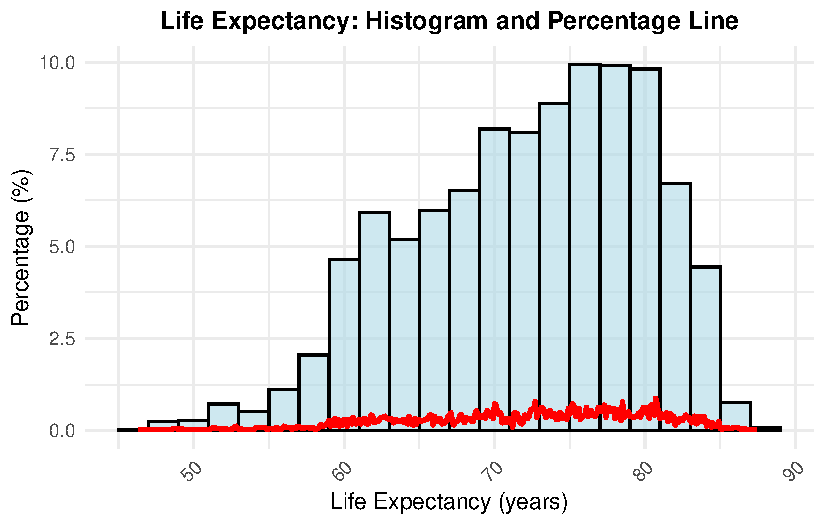
\includegraphics{paper_files/figure-pdf/fig-expectancy-1.pdf}

}

\caption{\label{fig-expectancy}This histogram shows the distribution of
the percentage of life expectancy. With a huge gap between 25 and 50, we
could indicate that most of the countries has a life expectancy of.
There exist large data with low life expectancy less than 25 years.}

\end{figure}%

\subsection{Predictor Variables}\label{predictor-variables}

The \textbf{predictor variables} (or independent variables) are the
factors believed to influence the life expectancy:

\begin{enumerate}
\def\labelenumi{\arabic{enumi}.}
\tightlist
\item
  \textbf{Income Group(\texttt{Income\_Group})}: The income group of a
  country is the key factor influencing the life expectancy. This
  variable provides context for comparing life expectancy between
  different levels of country income group. The division of the life
  expectancy by the income group of a country because income levels
  often correlate strongly with various factors affecting health and
  longevity. Higher income countries typically have more resources to
  invest in robust healthcare systems, with better living conditions
  while lower income countries often face challenges such as inadequate
  healthcare infrastructure and malnutrition.
\end{enumerate}

Following by the four income group, we would like to see the
distribution of the income group of 184 WHO member countries.
(\textbf{fid-income?}) shows that there are 55 countries at the high
income group, 26 countries at low income group, 54 countries at the
lower-middle group while there are 49 countries at the upper-middle
group. With significant less low income countries, we expect to see the
life expectancy lie in a comparably higher range. On the other hand,
there might exist sever outliers dropping the mean.

\begin{enumerate}
\def\labelenumi{\arabic{enumi}.}
\setcounter{enumi}{1}
\item
  \textbf{Gender(\texttt{Gender})}: The gender of the population of each
  country is included as a categorical variable (Male/Female/Both Sex).
  This is a key variable in the dataset because gender has been fully
  recognized connected with the biological physical factor which
  directly effect the life expectancy. Figure~\ref{fig-gender} shows
  that the with an stable average of 74, life expectancy of female is
  constantly higher than male's average of 70. The line plot reveals a
  steady increase until 2019, followed by a sharp decline in 2020, which
  is assumed to be associated with the impact of COVID-19.
\item
  \textbf{Region(Region)}: This is a categorical variable that
  classifies the geographic location of the countries. It is mapped one
  by one by the name of the country. The data is stored as the name of
  the continent(`Africa', `Oceania', `Asia', `Europe', `North America',
  `South America'). Figure~\ref{fig-region} indicates that with the
  number of 54, Africa has the most WHO member countries. Both Asia and
  Europe has 43 countries,listing in the middle while the other three
  continent has the significant less number of countries. North America
  has 22 countries, South America has 12 countries and Oceania has the
  least, 10 countries.
\end{enumerate}

\begin{figure}

\centering{

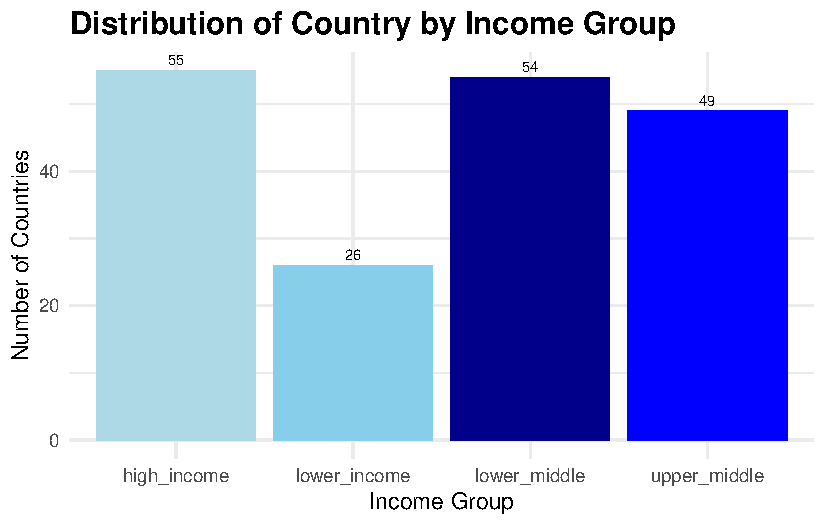
\includegraphics{paper_files/figure-pdf/fig-income-1.pdf}

}

\caption{\label{fig-income}Distribution of country income group.}

\end{figure}%

\begin{figure}

\centering{

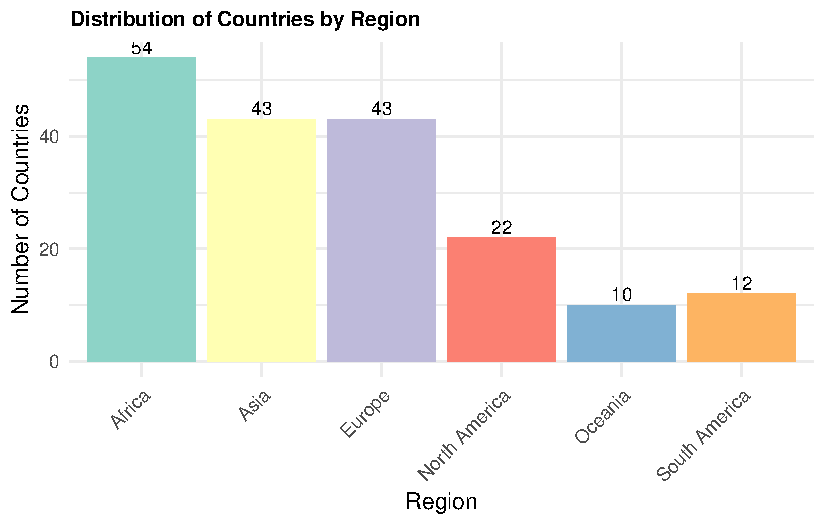
\includegraphics{paper_files/figure-pdf/fig-region-1.pdf}

}

\caption{\label{fig-region}Distribution of different region of the 184
countries. Africa has the most countries with an number of 54. Asia and
Europe has the same amount of 43, North America has 22 countries while
the other two continent has almost the same amount of countries.}

\end{figure}%

\begin{figure}

\centering{

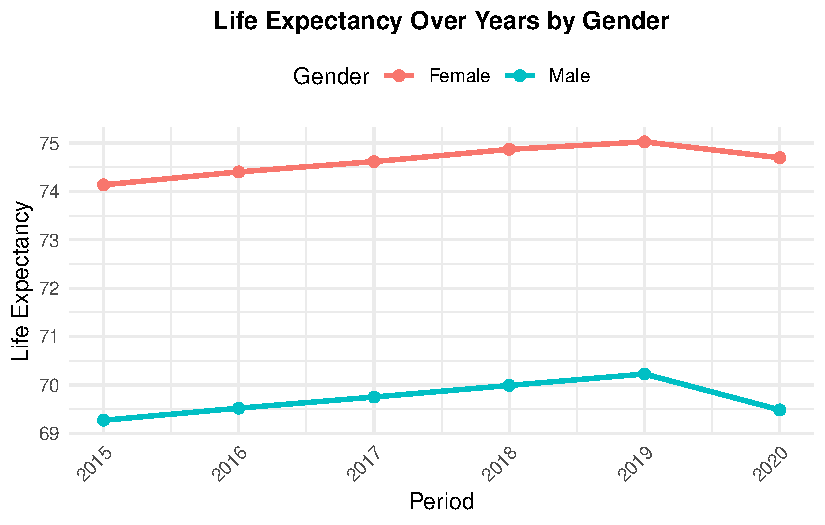
\includegraphics{paper_files/figure-pdf/fig-gender-1.pdf}

}

\caption{\label{fig-gender}Distribution of gender each year. The average
of female life expectancy is approximately 74 around years, constantly
higher than male's average of 70. Compared to male, female's life
expectancy is marginally more steady.}

\end{figure}%

\subsection{Basic Data Summary}\label{basic-data-summary}

The table below shows the basic summary of the mean, median, max,
standard deviation, variance and sample size of life expectancy. We
could tell that the average of the life expectancy from the 6 years is
45.9, with a large standard deviation of 26.9. The max of the life
expectancy is 87.4, among all 6624 rows of data. The standard deviation
and variance are extremely high because of the range of data is large,
in other words, because the mean and median are 45.9 and 37.7, compared
to the max 87.4, there is likely some outliers in the data creating such
a high standard deviation and variance.

\begin{figure}

\centering{

\begin{table}
\centering
\caption{Summary Statistics of Life Expectancy}
\centering
\begin{tabular}[t]{c|c|c|c|c|c}
\hline
Mean & Median & Max & Standard Deviation & Variance & N\\
\hline
45.9 & 37.7 & 87.4 & 26.9 & 724.2 & 6624\\
\hline
\end{tabular}
\end{table}

}

\caption{\label{fig-summary}Summary statistics of the number of life
expectancy over countries and years.}

\end{figure}%

\section{Model}\label{model}

\subsection{Model set-up}\label{sec-modset}

The goal of the Bayesian model is to incorporate prior knowledge, such
as insights from previous studies or analyses, into the selection of the
model. To predict the outcome of the life expectancy of people from
different regions, in this paper, we developed a linear regression
models using R (R Core Team 2023). The outcome variable,
\textbf{\texttt{Life\ Expectancy}}, is a continuous and represents the
average number of years a person is expected to live, assuming all
related resources remain constant throughout their lifetime. The model
aim to estimate and predict the life expectancy of people under
different gender, region and income group. The normal Gaussian
distribution is effective when used for modeling scenarios where the
residuals of the data are assumed to be independent nd normally
distributed around the regression line. The GAM allows for capturing
potential non-linear relationships between the predictors and the
outcome.

The model is specified as follows:

\begin{align} 
y_i|\mu_i, \sigma &\sim \text{Normal}(\mu_i, \sigma) \\
\mu_i &= \alpha + \beta_1 \text{Region}_i + \beta_2 \text{Gender}_i + \beta_3 \text{Income_Group}_i \\
\alpha &\sim \text{Normal}(0, 2.5) \\
\beta_1, \beta_2, \beta_3 &\sim \text{Normal}(0, 2.5) \\
\sigma &\sim \text{Exponential}(1)
\end{align}

Where:

\begin{itemize}
\item
  \(yi\) is the outcome variable (Life Expectancy)for the i-th
  observation.
\item
  \(\mu_i\): the linear predictor for life expectancy, including the
  intercept (\(\alpha\)) and the coefficients for the predictors Region,
  Country, Income Group, and Gender.
\item
  Priors for the intercept(\(\alpha\)) and the
  coefficients(\(\beta_1, \beta_2, \beta_3\)) are normal with mean 0 and
  standard deviation 2.5
\item
  \(\sigma\): the residual standard deviation, modeled as an exponential
  distribution with rate 1.
\end{itemize}

We run the model in R (R Core Team 2023) using the \texttt{rstanarm}
package of Goodrich et al. (2022). We use the default priors from
\texttt{rstanarm}. More explanation of the model could be found
Appendix~\ref{sec-model-details}.

\subsubsection{Model justification}\label{model-justification}

The linear regression model with Gaussian likelihood was chosen for this
analysis due to its simplicity and effectiveness in modeling continuous
outcome variables, such as life expectancy. Life expectancy is
influenced by multiple factors, including region, income group, and
gender. The linear model allows us to examine the average effect of each
predictor on the outcome, assuming that the relationships between these
predictors and life expectancy are linear.

The use of normal priors for the model coefficients \(\alpha\) and
\(\beta\) reflects a belief in prior knowledge that the true values of
these parameters are centered around zero, with some uncertainty, which
is consistent with standard Bayesian modeling practices. The prior scale
of 2.5 was chosen to reflect a reasonable level of uncertainty around
the estimates without being overly restrictive.

The Gaussian distribution was selected because life expectancy data, by
nature, is continuous and expected to follow a normal distribution. The
assumption of normal residuals is consistent with the idea that
deviations from the regression line are random and normally distributed,
allowing the model to make accurate inferences about the relationship
between predictors and the outcome.

Additionally, the exponential prior on the standard deviation \(\alpha\)
captures the residual variability in life expectancy across countries
and regions. The exponential distribution was chosen because it provides
a simple and interpretable way of modeling the variability, assuming
that the data are not heavily skewed.

This approach is appropriate given the data structure and the goal of
the analysis, which is to estimate and predict life expectancy across
different countries, regions, income groups, and genders. The model's
assumptions about the data, along with its priors, allow for robust
inference in the context of population health predictions.

\paragraph{Model Validation}\label{model-validation}

To assess the performance of the life expectancy prediction model, two
critical metrics were used: Root Mean Squared Error (RMSE) and
Out-of-Sample Testing. These methods help ensure that the model
generalizes well to unseen data and provides reliable predictions for
life expectancy across different regions, income groups, and genders.

RMSE measures the square root of the average squared differences between
the predicted and observed values. In the context of this model, RMSE
quantifies how closely the predicted life expectancy values align with
the actual observed values. Lower RMSE values indicate better model
performance, suggesting that the model's predictions are close to the
true values. The generalizability is checked by comparing rmse\_test and
rmse\_train. Seeing the test RMSE is slightly lower than the training
RMSE, the model generalizes well.

Out-of-Sample testing is a critical component of model evaluation. In
this approach, the data is split into a training set and a test set (or
holdout set). The training set is used to fit the model, while the test
set is used to evaluate how well the model performs on new, unseen data.
For this analysis, the model was trained using a portion of the data
(80\% of the dataset) and then evaluated on the remaining data (20\% of
the dataset) that was not used during training. This method allows us to
check whether the model overfits the training data or if it can
generalize well to unseen observations.

Together, RMSE and out-of-sample testing offer a robust framework for
model validation, ensuring that the predictions made by the life
expectancy model are both accurate and generalizable.

\begin{Shaded}
\begin{Highlighting}[]
\CommentTok{\#model\_developed \textless{}{-}}
  \CommentTok{\#readRDS(file = "\textasciitilde{}/lifeexpectancy/models/ledata\_normal\_model.rds")}

\CommentTok{\# Split the dataset into training and testing sets (80\% train, 20\% test)}
\CommentTok{\#set.seed(123)  \# Setting seed for reproducibility}
\CommentTok{\#train\_index \textless{}{-} createDataPartition(leab$\textasciigrave{}Life Expectancy\textasciigrave{}, p = 0.8, list = FALSE)}

\CommentTok{\#train\_data \textless{}{-} leab[train\_index, ]}
\CommentTok{\#test\_data \textless{}{-} leab[{-}train\_index, ]}

\CommentTok{\# Predict life expectancy using the test data}
\CommentTok{\#predictions \textless{}{-} predict(ledata\_normal\_model, newdata = test\_data)}
\end{Highlighting}
\end{Shaded}

\section{Results}\label{results}

\subsection{Overview of model results}\label{overview-of-model-results}

Our results are summarized in Table~\ref{tbl-modelresults}. We are
primarily interest in the

\subsection{Multiple linear regression
results}\label{multiple-linear-regression-results}

\section{Discussion}\label{discussion}

\subsection{Insights into different
gender}\label{insights-into-different-gender}

If my paper were 10 pages, then should be be at least 2.5 pages. The
discussion is a chance to show off what you know and what you learnt
from all this.

\subsection{Second discussion point}\label{second-discussion-point}

Please don't use these as sub-heading labels - change them to be what
your point actually is.

\subsection{Life Expectancy at 60}\label{life-expectancy-at-60}

The life expectancy at 60 means that how long is a person expected to
live at 60 instead of at birth.

\subsection{Weaknesses and next steps}\label{weaknesses-and-next-steps}

Weaknesses and next steps should also be included.

\newpage

\appendix

\section{Appendix}\label{sec-appendix}

\subsection{Data Cleaning Notes}\label{data-cleaning-notes}

We began by importing the raw dataset using the read\_csv function from
the tidyverse package. To focus our analysis on more relevant variables,
we selected specific columns, such as Indicator of life expectancy as
birth and life expectancy at 60 years, Country, Period, Gender, and Life
expectancy, omitting any unnecessary columns.

We functioned to extract the number before opening the square bracket of
life expectancy since the raw data gave both the range and the mean of
life expectancy of each country under each year.

We filter out the rows containing NA values in any of the selected
columns for reducing the noise and simpler further analysis.

We then renaming columns for clarity. For example, we changed `Location'
into `Country', ``Dim1'' for ``Gender'' and ``Value'' for ``Life
Expectancy'', making it easier for anyone working with the data to read
and understand what each variable represents.

Each column is rounded using the round function, specifying the desired
number of decimal places for each. Columns not mentioned in mutate
remain unchanged. This ensures a flexible and precise cleaning process
tailored to further comparison and graphing. We dropped the potential
percentage symbol to contain purely numerical data.

The income group column and the region column was not given in the raw
dataset. We created a new variable called ``Income\_Group'' by mapping
over country name to four income group (lower\_income, lower\_middle,
upper\_middle, high\_income) according to the index given by World Bank
Income Group. This is a key variable in predicting life expectancy since
it is believed that life expectancy is correlated to the income
situation. We as well made a mapping to the countries according to its
continent and saved as ``Region''. This is the variable indicates the
geographic context to the analysis. Countries are mapped into six
continents (``Africa'', ``Asia'', ``Europe'', ``North America'', ``South
America'', ``Oceania'') one by one.

We again merge the table, removing repeated columns and rows and mapping
the region and the country income under different given names.

Lastly, we filter out NAs again as a further check. We continue filter
out the Palestinian territory, which is not a country and was not mapped
in neither Region nor Income Group.

For easy reading format, we arrange the country into Alphabet order and
mutate the variables again for converting columns into appropriate data
types.

For easier visualization, we created four tables, which are grouped by
life expectancy at age 60, life expectancy at birth, life expectancy at
birth of Male and life expectancy at birth of Female.

After completing the cleaning, we saved the final dataset in both
Parquet and CSV formats for later analysis.

\subsection{Data Cleaning Table}\label{data-cleaning-table}

\begin{longtable}[]{@{}
  >{\raggedright\arraybackslash}p{(\columnwidth - 12\tabcolsep) * \real{0.2895}}
  >{\raggedright\arraybackslash}p{(\columnwidth - 12\tabcolsep) * \real{0.1754}}
  >{\raggedright\arraybackslash}p{(\columnwidth - 12\tabcolsep) * \real{0.0614}}
  >{\raggedright\arraybackslash}p{(\columnwidth - 12\tabcolsep) * \real{0.0965}}
  >{\raggedright\arraybackslash}p{(\columnwidth - 12\tabcolsep) * \real{0.1404}}
  >{\raggedright\arraybackslash}p{(\columnwidth - 12\tabcolsep) * \real{0.1140}}
  >{\raggedright\arraybackslash}p{(\columnwidth - 12\tabcolsep) * \real{0.1228}}@{}}

\caption{\label{tbl-cleaned_leab}Life expectancy over countries and
years}

\tabularnewline

\caption{Life Expectancy over countries and years (first 200
rows)}\tabularnewline
\toprule\noalign{}
\begin{minipage}[b]{\linewidth}\raggedright
Indicator
\end{minipage} & \begin{minipage}[b]{\linewidth}\raggedright
Country
\end{minipage} & \begin{minipage}[b]{\linewidth}\raggedright
Period
\end{minipage} & \begin{minipage}[b]{\linewidth}\raggedright
Gender
\end{minipage} & \begin{minipage}[b]{\linewidth}\raggedright
Life Expectancy
\end{minipage} & \begin{minipage}[b]{\linewidth}\raggedright
Income\_Group
\end{minipage} & \begin{minipage}[b]{\linewidth}\raggedright
Region
\end{minipage} \\
\midrule\noalign{}
\endfirsthead
\toprule\noalign{}
\begin{minipage}[b]{\linewidth}\raggedright
Indicator
\end{minipage} & \begin{minipage}[b]{\linewidth}\raggedright
Country
\end{minipage} & \begin{minipage}[b]{\linewidth}\raggedright
Period
\end{minipage} & \begin{minipage}[b]{\linewidth}\raggedright
Gender
\end{minipage} & \begin{minipage}[b]{\linewidth}\raggedright
Life Expectancy
\end{minipage} & \begin{minipage}[b]{\linewidth}\raggedright
Income\_Group
\end{minipage} & \begin{minipage}[b]{\linewidth}\raggedright
Region
\end{minipage} \\
\midrule\noalign{}
\endhead
\bottomrule\noalign{}
\endlastfoot
Life expectancy at birth (years) & Afghanistan & 2020 & Male & 59.3 &
lower\_income & Asia \\
Life expectancy at birth (years) & Afghanistan & 2020 & Both sexes &
60.5 & lower\_income & Asia \\
Life expectancy at birth (years) & Afghanistan & 2020 & Female & 61.7 &
lower\_income & Asia \\
Life expectancy at birth (years) & Afghanistan & 2019 & Male & 60.0 &
lower\_income & Asia \\
Life expectancy at birth (years) & Afghanistan & 2019 & Both sexes &
61.2 & lower\_income & Asia \\
Life expectancy at birth (years) & Afghanistan & 2019 & Female & 62.5 &
lower\_income & Asia \\
Life expectancy at birth (years) & Afghanistan & 2018 & Male & 59.0 &
lower\_income & Asia \\
Life expectancy at birth (years) & Afghanistan & 2018 & Both sexes &
60.5 & lower\_income & Asia \\
Life expectancy at birth (years) & Afghanistan & 2018 & Female & 62.1 &
lower\_income & Asia \\
Life expectancy at birth (years) & Afghanistan & 2017 & Male & 59.8 &
lower\_income & Asia \\
Life expectancy at birth (years) & Afghanistan & 2017 & Both sexes &
60.9 & lower\_income & Asia \\
Life expectancy at birth (years) & Afghanistan & 2017 & Female & 62.1 &
lower\_income & Asia \\
Life expectancy at birth (years) & Afghanistan & 2016 & Male & 59.2 &
lower\_income & Asia \\
Life expectancy at birth (years) & Afghanistan & 2016 & Both sexes &
60.4 & lower\_income & Asia \\
Life expectancy at birth (years) & Afghanistan & 2016 & Female & 61.7 &
lower\_income & Asia \\
Life expectancy at birth (years) & Afghanistan & 2015 & Male & 59.3 &
lower\_income & Asia \\
Life expectancy at birth (years) & Afghanistan & 2015 & Both sexes &
60.3 & lower\_income & Asia \\
Life expectancy at birth (years) & Afghanistan & 2015 & Female & 61.5 &
lower\_income & Asia \\
Life expectancy at birth (years) & Albania & 2020 & Male & 74.3 &
upper\_middle & Europe \\
Life expectancy at birth (years) & Albania & 2020 & Both sexes & 76.5 &
upper\_middle & Europe \\
Life expectancy at birth (years) & Albania & 2020 & Female & 79.0 &
upper\_middle & Europe \\
Life expectancy at birth (years) & Albania & 2019 & Male & 76.2 &
upper\_middle & Europe \\
Life expectancy at birth (years) & Albania & 2019 & Both sexes & 77.9 &
upper\_middle & Europe \\
Life expectancy at birth (years) & Albania & 2019 & Female & 79.9 &
upper\_middle & Europe \\
Life expectancy at birth (years) & Albania & 2018 & Male & 76.2 &
upper\_middle & Europe \\
Life expectancy at birth (years) & Albania & 2018 & Both sexes & 77.9 &
upper\_middle & Europe \\
Life expectancy at birth (years) & Albania & 2018 & Female & 79.9 &
upper\_middle & Europe \\
Life expectancy at birth (years) & Albania & 2017 & Male & 76.1 &
upper\_middle & Europe \\
Life expectancy at birth (years) & Albania & 2017 & Both sexes & 77.9 &
upper\_middle & Europe \\
Life expectancy at birth (years) & Albania & 2017 & Female & 79.9 &
upper\_middle & Europe \\
Life expectancy at birth (years) & Albania & 2016 & Male & 76.0 &
upper\_middle & Europe \\
Life expectancy at birth (years) & Albania & 2016 & Both sexes & 77.9 &
upper\_middle & Europe \\
Life expectancy at birth (years) & Albania & 2016 & Female & 79.9 &
upper\_middle & Europe \\
Life expectancy at birth (years) & Albania & 2015 & Male & 76.0 &
upper\_middle & Europe \\
Life expectancy at birth (years) & Albania & 2015 & Both sexes & 77.8 &
upper\_middle & Europe \\
Life expectancy at birth (years) & Albania & 2015 & Female & 79.6 &
upper\_middle & Europe \\
Life expectancy at birth (years) & Algeria & 2020 & Male & 73.0 &
lower\_middle & Africa \\
Life expectancy at birth (years) & Algeria & 2020 & Both sexes & 74.0 &
lower\_middle & Africa \\
Life expectancy at birth (years) & Algeria & 2020 & Female & 75.2 &
lower\_middle & Africa \\
Life expectancy at birth (years) & Algeria & 2019 & Male & 76.2 &
lower\_middle & Africa \\
Life expectancy at birth (years) & Algeria & 2019 & Both sexes & 76.5 &
lower\_middle & Africa \\
Life expectancy at birth (years) & Algeria & 2019 & Female & 77.1 &
lower\_middle & Africa \\
Life expectancy at birth (years) & Algeria & 2018 & Male & 76.1 &
lower\_middle & Africa \\
Life expectancy at birth (years) & Algeria & 2018 & Both sexes & 76.4 &
lower\_middle & Africa \\
Life expectancy at birth (years) & Algeria & 2018 & Female & 77.0 &
lower\_middle & Africa \\
Life expectancy at birth (years) & Algeria & 2017 & Male & 76.0 &
lower\_middle & Africa \\
Life expectancy at birth (years) & Algeria & 2017 & Both sexes & 76.4 &
lower\_middle & Africa \\
Life expectancy at birth (years) & Algeria & 2017 & Female & 77.0 &
lower\_middle & Africa \\
Life expectancy at birth (years) & Algeria & 2016 & Male & 75.9 &
lower\_middle & Africa \\
Life expectancy at birth (years) & Algeria & 2016 & Both sexes & 76.3 &
lower\_middle & Africa \\
Life expectancy at birth (years) & Algeria & 2016 & Female & 76.8 &
lower\_middle & Africa \\
Life expectancy at birth (years) & Algeria & 2015 & Male & 75.8 &
lower\_middle & Africa \\
Life expectancy at birth (years) & Algeria & 2015 & Both sexes & 76.1 &
lower\_middle & Africa \\
Life expectancy at birth (years) & Algeria & 2015 & Female & 76.6 &
lower\_middle & Africa \\
Life expectancy at birth (years) & Angola & 2020 & Male & 60.4 &
lower\_middle & Africa \\
Life expectancy at birth (years) & Angola & 2020 & Both sexes & 62.6 &
lower\_middle & Africa \\
Life expectancy at birth (years) & Angola & 2020 & Female & 64.9 &
lower\_middle & Africa \\
Life expectancy at birth (years) & Angola & 2019 & Male & 60.3 &
lower\_middle & Africa \\
Life expectancy at birth (years) & Angola & 2019 & Both sexes & 62.5 &
lower\_middle & Africa \\
Life expectancy at birth (years) & Angola & 2019 & Female & 64.7 &
lower\_middle & Africa \\
Life expectancy at birth (years) & Angola & 2018 & Male & 60.1 &
lower\_middle & Africa \\
Life expectancy at birth (years) & Angola & 2018 & Both sexes & 62.3 &
lower\_middle & Africa \\
Life expectancy at birth (years) & Angola & 2018 & Female & 64.5 &
lower\_middle & Africa \\
Life expectancy at birth (years) & Angola & 2017 & Male & 59.8 &
lower\_middle & Africa \\
Life expectancy at birth (years) & Angola & 2017 & Both sexes & 62.0 &
lower\_middle & Africa \\
Life expectancy at birth (years) & Angola & 2017 & Female & 64.3 &
lower\_middle & Africa \\
Life expectancy at birth (years) & Angola & 2016 & Male & 59.5 &
lower\_middle & Africa \\
Life expectancy at birth (years) & Angola & 2016 & Both sexes & 61.8 &
lower\_middle & Africa \\
Life expectancy at birth (years) & Angola & 2016 & Female & 64.2 &
lower\_middle & Africa \\
Life expectancy at birth (years) & Angola & 2015 & Male & 59.1 &
lower\_middle & Africa \\
Life expectancy at birth (years) & Angola & 2015 & Both sexes & 61.6 &
lower\_middle & Africa \\
Life expectancy at birth (years) & Angola & 2015 & Female & 64.1 &
lower\_middle & Africa \\
Life expectancy at birth (years) & Antigua and Barbuda & 2020 & Male &
75.6 & high\_income & North America \\
Life expectancy at birth (years) & Antigua and Barbuda & 2020 & Both
sexes & 77.6 & high\_income & North America \\
Life expectancy at birth (years) & Antigua and Barbuda & 2020 & Female &
79.4 & high\_income & North America \\
Life expectancy at birth (years) & Antigua and Barbuda & 2019 & Male &
74.0 & high\_income & North America \\
Life expectancy at birth (years) & Antigua and Barbuda & 2019 & Both
sexes & 75.7 & high\_income & North America \\
Life expectancy at birth (years) & Antigua and Barbuda & 2019 & Female &
77.1 & high\_income & North America \\
Life expectancy at birth (years) & Antigua and Barbuda & 2018 & Male &
74.0 & high\_income & North America \\
Life expectancy at birth (years) & Antigua and Barbuda & 2018 & Both
sexes & 75.6 & high\_income & North America \\
Life expectancy at birth (years) & Antigua and Barbuda & 2018 & Female &
77.0 & high\_income & North America \\
Life expectancy at birth (years) & Antigua and Barbuda & 2017 & Male &
73.9 & high\_income & North America \\
Life expectancy at birth (years) & Antigua and Barbuda & 2017 & Both
sexes & 75.6 & high\_income & North America \\
Life expectancy at birth (years) & Antigua and Barbuda & 2017 & Female &
77.0 & high\_income & North America \\
Life expectancy at birth (years) & Antigua and Barbuda & 2016 & Male &
73.8 & high\_income & North America \\
Life expectancy at birth (years) & Antigua and Barbuda & 2016 & Both
sexes & 75.5 & high\_income & North America \\
Life expectancy at birth (years) & Antigua and Barbuda & 2016 & Female &
77.1 & high\_income & North America \\
Life expectancy at birth (years) & Antigua and Barbuda & 2015 & Male &
73.8 & high\_income & North America \\
Life expectancy at birth (years) & Antigua and Barbuda & 2015 & Both
sexes & 75.6 & high\_income & North America \\
Life expectancy at birth (years) & Antigua and Barbuda & 2015 & Female &
77.2 & high\_income & North America \\
Life expectancy at birth (years) & Argentina & 2020 & Male & 73.1 &
upper\_middle & South America \\
Life expectancy at birth (years) & Argentina & 2020 & Both sexes & 76.2
& upper\_middle & South America \\
Life expectancy at birth (years) & Argentina & 2020 & Female & 79.4 &
upper\_middle & South America \\
Life expectancy at birth (years) & Argentina & 2019 & Male & 74.0 &
upper\_middle & South America \\
Life expectancy at birth (years) & Argentina & 2019 & Both sexes & 77.0
& upper\_middle & South America \\
Life expectancy at birth (years) & Argentina & 2019 & Female & 79.9 &
upper\_middle & South America \\
Life expectancy at birth (years) & Argentina & 2018 & Male & 73.7 &
upper\_middle & South America \\
Life expectancy at birth (years) & Argentina & 2018 & Both sexes & 76.9
& upper\_middle & South America \\
Life expectancy at birth (years) & Argentina & 2018 & Female & 79.9 &
upper\_middle & South America \\
Life expectancy at birth (years) & Argentina & 2017 & Male & 73.6 &
upper\_middle & South America \\
Life expectancy at birth (years) & Argentina & 2017 & Both sexes & 76.6
& upper\_middle & South America \\
Life expectancy at birth (years) & Argentina & 2017 & Female & 79.6 &
upper\_middle & South America \\
Life expectancy at birth (years) & Argentina & 2016 & Male & 73.0 &
upper\_middle & South America \\
Life expectancy at birth (years) & Argentina & 2016 & Both sexes & 76.1
& upper\_middle & South America \\
Life expectancy at birth (years) & Argentina & 2016 & Female & 79.2 &
upper\_middle & South America \\
Life expectancy at birth (years) & Argentina & 2015 & Male & 73.3 &
upper\_middle & South America \\
Life expectancy at birth (years) & Argentina & 2015 & Both sexes & 76.5
& upper\_middle & South America \\
Life expectancy at birth (years) & Argentina & 2015 & Female & 79.6 &
upper\_middle & South America \\
Life expectancy at birth (years) & Armenia & 2020 & Male & 62.7 &
upper\_middle & Europe \\
Life expectancy at birth (years) & Armenia & 2020 & Both sexes & 69.3 &
upper\_middle & Europe \\
Life expectancy at birth (years) & Armenia & 2020 & Female & 76.2 &
upper\_middle & Europe \\
Life expectancy at birth (years) & Armenia & 2019 & Male & 70.8 &
upper\_middle & Europe \\
Life expectancy at birth (years) & Armenia & 2019 & Both sexes & 75.7 &
upper\_middle & Europe \\
Life expectancy at birth (years) & Armenia & 2019 & Female & 79.8 &
upper\_middle & Europe \\
Life expectancy at birth (years) & Armenia & 2018 & Male & 71.0 &
upper\_middle & Europe \\
Life expectancy at birth (years) & Armenia & 2018 & Both sexes & 75.6 &
upper\_middle & Europe \\
Life expectancy at birth (years) & Armenia & 2018 & Female & 79.5 &
upper\_middle & Europe \\
Life expectancy at birth (years) & Armenia & 2017 & Male & 70.6 &
upper\_middle & Europe \\
Life expectancy at birth (years) & Armenia & 2017 & Both sexes & 75.2 &
upper\_middle & Europe \\
Life expectancy at birth (years) & Armenia & 2017 & Female & 79.1 &
upper\_middle & Europe \\
Life expectancy at birth (years) & Armenia & 2016 & Male & 69.8 &
upper\_middle & Europe \\
Life expectancy at birth (years) & Armenia & 2016 & Both sexes & 74.4 &
upper\_middle & Europe \\
Life expectancy at birth (years) & Armenia & 2016 & Female & 78.5 &
upper\_middle & Europe \\
Life expectancy at birth (years) & Armenia & 2015 & Male & 69.8 &
upper\_middle & Europe \\
Life expectancy at birth (years) & Armenia & 2015 & Both sexes & 74.3 &
upper\_middle & Europe \\
Life expectancy at birth (years) & Armenia & 2015 & Female & 78.3 &
upper\_middle & Europe \\
Life expectancy at birth (years) & Australia & 2020 & Male & 81.5 &
high\_income & Oceania \\
Life expectancy at birth (years) & Australia & 2020 & Both sexes & 83.4
& high\_income & Oceania \\
Life expectancy at birth (years) & Australia & 2020 & Female & 85.2 &
high\_income & Oceania \\
Life expectancy at birth (years) & Australia & 2019 & Male & 80.7 &
high\_income & Oceania \\
Life expectancy at birth (years) & Australia & 2019 & Both sexes & 82.6
& high\_income & Oceania \\
Life expectancy at birth (years) & Australia & 2019 & Female & 84.6 &
high\_income & Oceania \\
Life expectancy at birth (years) & Australia & 2018 & Male & 81.2 &
high\_income & Oceania \\
Life expectancy at birth (years) & Australia & 2018 & Both sexes & 83.0
& high\_income & Oceania \\
Life expectancy at birth (years) & Australia & 2018 & Female & 84.9 &
high\_income & Oceania \\
Life expectancy at birth (years) & Australia & 2017 & Male & 80.8 &
high\_income & Oceania \\
Life expectancy at birth (years) & Australia & 2017 & Both sexes & 82.7
& high\_income & Oceania \\
Life expectancy at birth (years) & Australia & 2017 & Female & 84.5 &
high\_income & Oceania \\
Life expectancy at birth (years) & Australia & 2016 & Male & 80.7 &
high\_income & Oceania \\
Life expectancy at birth (years) & Australia & 2016 & Both sexes & 82.6
& high\_income & Oceania \\
Life expectancy at birth (years) & Australia & 2016 & Female & 84.5 &
high\_income & Oceania \\
Life expectancy at birth (years) & Australia & 2015 & Male & 80.4 &
high\_income & Oceania \\
Life expectancy at birth (years) & Australia & 2015 & Both sexes & 82.3
& high\_income & Oceania \\
Life expectancy at birth (years) & Australia & 2015 & Female & 84.2 &
high\_income & Oceania \\
Life expectancy at birth (years) & Austria & 2020 & Male & 78.8 &
high\_income & Europe \\
Life expectancy at birth (years) & Austria & 2020 & Both sexes & 81.1 &
high\_income & Europe \\
Life expectancy at birth (years) & Austria & 2020 & Female & 83.3 &
high\_income & Europe \\
Life expectancy at birth (years) & Austria & 2019 & Male & 79.4 &
high\_income & Europe \\
Life expectancy at birth (years) & Austria & 2019 & Both sexes & 81.6 &
high\_income & Europe \\
Life expectancy at birth (years) & Austria & 2019 & Female & 83.8 &
high\_income & Europe \\
Life expectancy at birth (years) & Austria & 2018 & Male & 79.2 &
high\_income & Europe \\
Life expectancy at birth (years) & Austria & 2018 & Both sexes & 81.4 &
high\_income & Europe \\
Life expectancy at birth (years) & Austria & 2018 & Female & 83.6 &
high\_income & Europe \\
Life expectancy at birth (years) & Austria & 2017 & Male & 79.2 &
high\_income & Europe \\
Life expectancy at birth (years) & Austria & 2017 & Both sexes & 81.4 &
high\_income & Europe \\
Life expectancy at birth (years) & Austria & 2017 & Female & 83.5 &
high\_income & Europe \\
Life expectancy at birth (years) & Austria & 2016 & Male & 79.1 &
high\_income & Europe \\
Life expectancy at birth (years) & Austria & 2016 & Both sexes & 81.4 &
high\_income & Europe \\
Life expectancy at birth (years) & Austria & 2016 & Female & 83.6 &
high\_income & Europe \\
Life expectancy at birth (years) & Austria & 2015 & Male & 78.6 &
high\_income & Europe \\
Life expectancy at birth (years) & Austria & 2015 & Both sexes & 81.0 &
high\_income & Europe \\
Life expectancy at birth (years) & Austria & 2015 & Female & 83.3 &
high\_income & Europe \\
Life expectancy at birth (years) & Azerbaijan & 2020 & Male & 67.5 &
upper\_middle & Europe \\
Life expectancy at birth (years) & Azerbaijan & 2020 & Both sexes & 71.4
& upper\_middle & Europe \\
Life expectancy at birth (years) & Azerbaijan & 2020 & Female & 75.5 &
upper\_middle & Europe \\
Life expectancy at birth (years) & Azerbaijan & 2019 & Male & 73.4 &
upper\_middle & Europe \\
Life expectancy at birth (years) & Azerbaijan & 2019 & Both sexes & 75.8
& upper\_middle & Europe \\
Life expectancy at birth (years) & Azerbaijan & 2019 & Female & 78.1 &
upper\_middle & Europe \\
Life expectancy at birth (years) & Azerbaijan & 2018 & Male & 72.6 &
upper\_middle & Europe \\
Life expectancy at birth (years) & Azerbaijan & 2018 & Both sexes & 75.1
& upper\_middle & Europe \\
Life expectancy at birth (years) & Azerbaijan & 2018 & Female & 77.5 &
upper\_middle & Europe \\
Life expectancy at birth (years) & Azerbaijan & 2017 & Male & 72.2 &
upper\_middle & Europe \\
Life expectancy at birth (years) & Azerbaijan & 2017 & Both sexes & 74.6
& upper\_middle & Europe \\
Life expectancy at birth (years) & Azerbaijan & 2017 & Female & 76.9 &
upper\_middle & Europe \\
Life expectancy at birth (years) & Azerbaijan & 2016 & Male & 71.8 &
upper\_middle & Europe \\
Life expectancy at birth (years) & Azerbaijan & 2016 & Both sexes & 74.0
& upper\_middle & Europe \\
Life expectancy at birth (years) & Azerbaijan & 2016 & Female & 76.0 &
upper\_middle & Europe \\
Life expectancy at birth (years) & Azerbaijan & 2015 & Male & 71.7 &
upper\_middle & Europe \\
Life expectancy at birth (years) & Azerbaijan & 2015 & Both sexes & 73.6
& upper\_middle & Europe \\
Life expectancy at birth (years) & Azerbaijan & 2015 & Female & 75.5 &
upper\_middle & Europe \\
Life expectancy at birth (years) & Bahamas & 2020 & Male & 69.2 &
high\_income & North America \\
Life expectancy at birth (years) & Bahamas & 2020 & Both sexes & 72.6 &
high\_income & North America \\
Life expectancy at birth (years) & Bahamas & 2020 & Female & 76.0 &
high\_income & North America \\
Life expectancy at birth (years) & Bahamas & 2019 & Male & 68.1 &
high\_income & North America \\
Life expectancy at birth (years) & Bahamas & 2019 & Both sexes & 70.7 &
high\_income & North America \\
Life expectancy at birth (years) & Bahamas & 2019 & Female & 73.3 &
high\_income & North America \\
Life expectancy at birth (years) & Bahamas & 2018 & Male & 70.2 &
high\_income & North America \\
Life expectancy at birth (years) & Bahamas & 2018 & Both sexes & 73.4 &
high\_income & North America \\
Life expectancy at birth (years) & Bahamas & 2018 & Female & 76.5 &
high\_income & North America \\
Life expectancy at birth (years) & Bahamas & 2017 & Male & 70.0 &
high\_income & North America \\
Life expectancy at birth (years) & Bahamas & 2017 & Both sexes & 73.2 &
high\_income & North America \\
Life expectancy at birth (years) & Bahamas & 2017 & Female & 76.3 &
high\_income & North America \\
Life expectancy at birth (years) & Bahamas & 2016 & Male & 69.7 &
high\_income & North America \\
Life expectancy at birth (years) & Bahamas & 2016 & Both sexes & 72.9 &
high\_income & North America \\
Life expectancy at birth (years) & Bahamas & 2016 & Female & 76.1 &
high\_income & North America \\
Life expectancy at birth (years) & Bahamas & 2015 & Male & 69.8 &
high\_income & North America \\
Life expectancy at birth (years) & Bahamas & 2015 & Both sexes & 72.9 &
high\_income & North America \\
Life expectancy at birth (years) & Bahamas & 2015 & Female & 76.0 &
high\_income & North America \\
Life expectancy at birth (years) & Bahrain & 2020 & Male & 73.6 &
high\_income & Asia \\
Life expectancy at birth (years) & Bahrain & 2020 & Both sexes & 74.9 &
high\_income & Asia \\

\end{longtable}

\subsection{Idealized Survey}\label{idealized-survey}

\textbf{Survey: Life Expectancy and Lifestyle Survey}

Thank you for participating in this survey. This survey aims to gather
insights into the factors influencing life expectancy, including gender,
region and income group. Your responses will help us understand
individual perspectives and experience towards national policy.
Participation is voluntary, and your answers will remain anonymous.

\textbf{Contact Information:} If you have any questions about the survey
or the data collection process, please contact

\textbf{Survey Coordinator}: Yanfei Huang\\
\textbf{Email}: yanfei.huang@mail.utoronto.ca

\textbf{Section 1: Demographics}

\textbf{1. Gender}

\begin{itemize}
\tightlist
\item
  Male
\item
  Female
\item
  Non-binary
\item
  Prefer not to say
\end{itemize}

\textbf{2. Age (in years)}

Please write the number: \_\_\_\_\_\_

\textbf{3. Region of Residence}

\begin{itemize}
\tightlist
\item
  Africa
\item
  Asia
\item
  Europe
\item
  North America
\item
  South America
\item
  Oceania
\end{itemize}

\textbf{4. Income Level}

Annual Income (Optional): \_\_\_\_\_\_ USD

Income Group: - Low Income (Less than \$1,000/year) - Lower-Middle
Income (\$1,001 - \$10,000/year) - Upper-Middle Income (\$10,001 -
\$50,000/year) - High Income (More than \$50,000/year)

\textbf{Section 2: Health and Lifestyle}

\textbf{5. Current Life Expectancy Perception}

How many years do you expect to live?

Please write the number: \_\_\_\_\_\_

\textbf{6. Healthcare Access}

How often do you visit healthcare professionals - Regularly (e.g.,
annual checkups) - Occasionally (e.g., only when unwell) - Rarely or
Never

\textbf{7. Dietary Habits}

How would you describe your diet?

\begin{itemize}
\tightlist
\item
  Balanced and healthy
\item
  Somewhat balanced
\item
  Unhealthy
\end{itemize}

\textbf{8. Physical Activity}

How many hours of physical activity do you engage in per week? - Less
than 1 hour - 1-3 hours - More than 3 hours

\textbf{9. Smoking Habits}

Do you smoke? - Yes - No

\textbf{10. Alcohol Consumption}

How often do you consume alcoholic beverages? - Never - Occasionally
(e.g., social drinking) - Frequently

\textbf{Section 3: Environmental and Social Factors}

\textbf{11.Living Environment}

How would you describe your living area? - Urban - Suburban - Rural

\textbf{Final Section}

Thank you for completing this survey! Your responses will help capture
information about economic conditions, access to healthcare and
education, and basic living standards, which are critical for
understanding life expectancy predictors and the impact of socioeconomic
factors on health outcomes.

\section{Additional data details}\label{additional-data-details}

\subsection{Model details}\label{sec-model-details}

The model developed for predicting life expectancy is a linear
regression model, where the goal is to estimate the outcome variable,
Life Expectancy, based on multiple predictors: Region, Income Group, and
Gender. Here's a more detailed breakdown of the components and structure
of the model:

\textbf{1. Outcome variable (yi)}

The outcome variable \(y_i\) represents the life expectancy of an
country. This is a continuous variable representing the number of years
a person is expected to live, assuming all conditions remain constant.

\textbf{2. Linear Predictor (μi)}

The linear predictor \(μ_i\) is a linear combination of the predictors,
which includes an intercept term \(α\) and the coefficients \(β_1\),
\(β_2\), \(β_3\), corresponding to Region, Income Group, and Gender,
respectively. This linear equation models the relationship between life
expectancy and the predictors
\(\mu_i = \alpha + \beta_1(Region) + \beta_2(Income Group) + \beta_3 (Gender)\)
The values for these coefficients (betas) represent the expected change
in life expectancy for a one-unit change in each respective predictor.

\textbf{3. Priors}

The prior distribution for the intercept \(α\) and the coefficients
\(β_1\), \(β_2\), \(β_3\) is assumed to be normal with a mean of 0 and a
standard deviation of 2.5. This reflects our belief that, prior to
seeing the data, the intercept and coefficients are most likely close to
0, with a reasonable range of variability (the scale of 2.5 is
relatively broad, allowing flexibility in fitting the model).

The prior for \(σ\) (residual standard deviation) is assumed to follow
an exponential distribution with a rate of 1. This prior reflects the
assumption that the variance of the residuals (i.e., the deviation of
the actual observations from the predicted values) is positive and that
it could reasonably be spread across a wide range of values.

\textbf{4. Residual Standard Deviation (σ)} The model also estimates
\(σ\), which represents the standard deviation of the residuals --- the
errors between the observed life expectancy values and those predicted
by the model. The prior for \(σ\) is assumed to follow an exponential
distribution with a rate of 1, meaning that smaller values of \(σ\)
(indicating less variation) are somewhat more likely than larger ones.

\textbf{5. Gaussian Likelihood} The outcome variable Life Expectancy is
modeled using a normal distribution with mean μi (the linear predictor)
and standard deviation σ. This means that the residuals (the differences
between the observed and predicted values) are assumed to be normally
distributed: \(y_i| \mu_i, \sigma ~ Normal(\mu_i, \sigma)\) This is a
typical assumption in regression models when the data is continuous, and
the relationship between the predictors and the outcome is linear.

\subsection{RMSE Full table}\label{rmse-full-table}

\subsection{Additional graph for
analysis}\label{additional-graph-for-analysis}

\newpage

\section*{References}\label{references}
\addcontentsline{toc}{section}{References}

\phantomsection\label{refs}
\begin{CSLReferences}{1}{0}
\bibitem[\citeproctext]{ref-rstanarm}
Goodrich, Ben, Jonah Gabry, Imad Ali, and Sam Brilleman. 2022.
{``{rstanarm: {Bayesian} applied regression modeling via {Stan}}.''}
\url{https://mc-stan.org/rstanarm/}.

\bibitem[\citeproctext]{ref-citeR}
R Core Team. 2023. \emph{{R: A Language and Environment for Statistical
Computing}}. Vienna, Austria: R Foundation for Statistical Computing.
\url{https://www.R-project.org/}.

\end{CSLReferences}




\end{document}
